\documentclass{acm_proc_article-sp}

\usepackage{bytefield}

\begin{document}

\title{Routing algorithms in the Internet}

\author{
  Paleshnikov, Nikolay\\
 \affaddr{RWTH Aachen}\\
  \texttt{nikolay.paleshnikov@rwth-aachen.de}
  \and
  Witt, Markus\\
 \affaddr{RWTH Aachen}\\
  \texttt{markus.witt@rwth-aachen.de}
}

\date{\today}

\maketitle
\begin{abstract}

The subject of this paper is to place routing in the context of the contemporary Internet and then outline some of the most widely used approaches applied in the state-of-art routing algorithms. Then a more detailed study of the hiearchy of routing algorithms will be presented concerning OSPF and BGP. Some problems arising from mobility and vulnerability of the network structure and their possible solutions will be the topic of the last section of the current paper.   

\end{abstract}

\keywords{Internet, Routing, OSPF, BGP, MANET} 

\section{Introduction}

One of the most challenging tasks in a network is how to providereliable and fast interconnectivity between its multiple hosts. Most of the complexity undelying that problem is implemented in the network layer of the protocol stack. Its instances include not only the hosts, but also the intersection points (routers) of the network. As the Internet only provides a connectionless service at its network layer, specific paths must be chosen for each information entity (datagram) to be transported. Routing attempts on finding the most efficient path between source and destination of the data flow using unique identifiers such as their IP-adresses.

In big enterprise networks consisting of multiple subnets, static configuration of routes will prove inefficient. It also requires manual reconfiguration in case of a hardware failure. Therefore, dynamic routing is mostly employed. Since hosts are usually connected to a single router, the tough decisions fall on the routers in between them. These decisions must be done in a deterministic way following the steps specified by a routing algorithm. The computed routes must be stored in a routing table indexed by the destination host, enabling fast look-up of the next-hop router upon a datagram arrival. The routing algorithm should also be able to respond fast to changes in topology and disseminate crucial information about the network state periodically (via broadcast).

With a network growing as fast as the Internet, scalability becomes a major factor for the success of employing a specific solution to the problems stated above. Therefore, a hierarchy of routing algorithms is urgent. From an architectural point of view, the fundament is based on multiple interior gateway protocols (IGPs), responsible for the datagram transportation within a single autonomous system (AS), on top of which an unified exterior gateway protocol (EGP) is executed so as to interconnect their functionality and form a coherent network structure. The IGPs will be the topic of section 2, whereas the EGP will be discussed in section 3 of this paper.

\section{Interior Gateway Protocols}

It will be useful to outline some of the basic principles employed by all of the interior routing algorithms in the first place. Discussions on this issue can be found in either \cite{kurose} or \cite{tanenbaum}. Firstly, the whole network is modelled as a weighted directed graph. The weights of the edges might represent the delay, bandwidth or cost of a single link between two routers and are taken into account for the determinition of a good path for every source-destination pair. Since the weights of both edges connecting two routers in opposite directions need not be identical, the most efficient paths between a pair of nodes are rarely symetrical. Secondly, the optimality principle states that if the most efficient path from router A to router C goes through router B, then the optimal route from B to C also falls along the same path. This principle is extensively used when we do not have a complete view of the whole network, such being the case with a decentralized routing algorithm.

\subsection{Distance-Vector Routing}

The distance-vector routing algorithms fall into exactly that category. The following review is based mostly on \cite{kurose}. In a distance-vector routing algorithm, each node maintains information only about its direct neighbours in a data structure called a distance vector (DV). For the need of computing best routes to all of the other nodes in the network, DV are propagated among adjascent routers, what makes every DV algorithm a distributed one. To secure reliability against topological changes such as a link or a router failure, the information exchange must take place at well-defined time intervals in an iterative manner. After receiving a new DV from some of its neighbours, each node must update its own DV according to the Bellmann-Ford equation: \begin{equation*} d_{x}(y) = min_{v}\{c(x,v)+d_{v}(y)\} \end{equation*} in which $d_{x}(y)$ denotes the least-cost path from x to y, v an arbitrary neighbour of x, c(x,v) the weight of the link between x and v and $d_{v}(y)$ the least-cost path from v to y, respectively. This equation is evidently based on the optimality principle indicated above and computes $d_{x}(y)$ with a time complexity of $\mathcal{O}(|v|)$ , where |v| represents the number of neighbours of x.

While DV algorithms have some aparent advantages such as the space efficiency of the routing tables maintained and the littme amount of information processed at the nodes of the network, a deeper analysis of their behaviour reveals a few insurmountable drawbacks, as pointed out in \cite{huitema}. The bouncing effect occurs in case of a sudden link failure. Consider the scenario described in Figure 1. In the beginning, the optimal routes to C are computed to cost 1 from B and 2 from A (through B). If the link between B and C breaks, the cost of the route from B to C will initially be set to infinity and then updated to 3 regarding the incoming DV of A, which advertises a shortest path to C at the cost 2. At that point, an undetectable loop is taking place between A and B. Since the view of the network structure at each node is limited to its direct neighbours, it does not know through which nodes its routes go along their way to the destination. A convergence to a stable state will be achieved after the exchange of seven more DVs, as A will finally set its optimal route to C through the link costing 10. In the meanwhile, datagrams will loop until their Time to live expires, possibly causing congestion on the links comprising the loop. Because DV interchange relies on those links, the recovery from a link failure may be further slowed down.

\begin{figure}
\centering
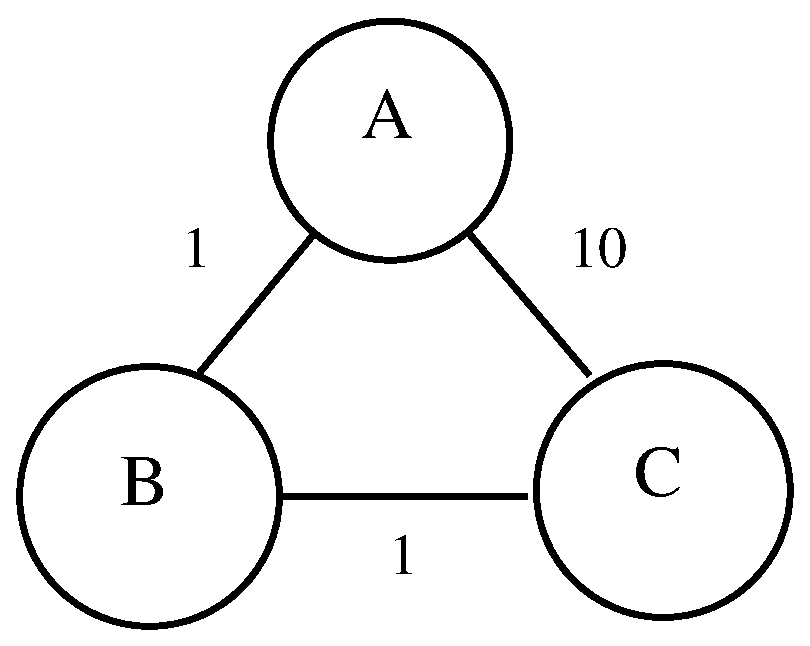
\epsfig{file=Diagram1.eps, height=1.8in, width=2.3in}
\caption{Bouncing Effect}
\end{figure}

A special case of the bouncing effect, also known as the count-to-infinity problem, is the result of a break-down of a bridge in the graph, i.e. a link representing the sole connection to the rest of the network. Supposed that the link marked with * in Figure 2 was torn down, the bouncing effect between nodes A and B in their attempt to compute best-cost path to C, as well as between C, D and E in their struggle to resolve an optimal route to A, will endure infinitely. The definition of a number slighly bigger than the diameter of the network as infinity solves that issue. Beyond that number, no further computations of the cost to a specific node are undertaken. 

\begin{figure}
\centering
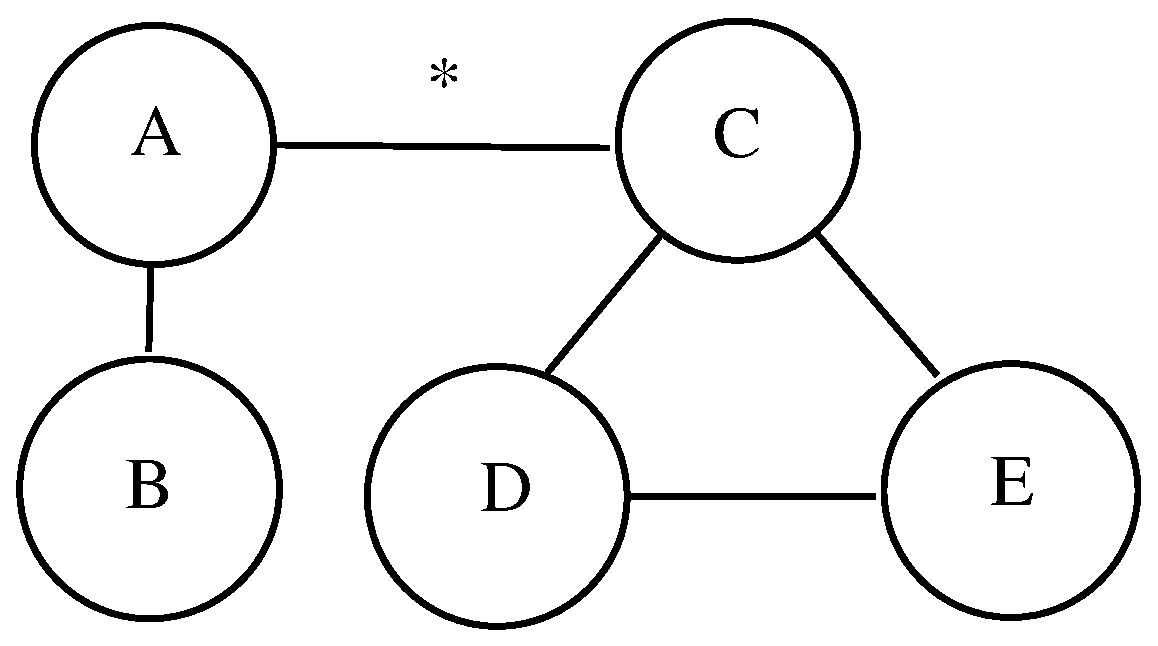
\epsfig{file=Diagram2.eps, height=1.8in, width=3.5in}
\caption{Count-to-infinity Problem}
\end{figure}

To directly prevent the cause of the bouncing effect between two nodes, a technique called split horizon may be applied. It states that B should not announce a route reaching C to A, since it has determined a to be the next-hop router to C in its routing table. Despite its simplicity, split horizon is not ground-breaking for its inablility to break loop of higher order such as the one between nodes C, D and E in Figure 2.  

A distance-vector algorithm also suffers from a certain lack of robustness. Provided that a node broadcasted an incorrect link cost to its neighbours, they would not have any database to compare this cost with and would have to blindly accept it. The numerous disadvantages of DV routing have led to the development of a fundamentally different approach to intra-AS routing, called link-state routing.

\subsection{Link-State Routing}

The link-state (LS) routing algorithms need complete information about all of the link costs in the network and are therefore often described as global routing algorithms. The computations they perform are based on the widely known Dijkstra's algorithm, solving the single-source shortest path problem for a given Graph G = (V, E). It operates by means of a set of nodes N to which it has already assigned a shortest path, which initially consists solely of the source node s. During its execution it also maintains a table with the best known distances to D(x,y) for every pair of nodes x and y, initialized as the link costs (edge weights c(x,y)) if a direct connection is present and as infinity otherwise. In each step of the following loop, it chooses the node $t \in V \setminus N$ with the minimum distance from the source D(s,t), updates the distances from the source to each of t's neighbours regarding the equation  \begin{equation*} D(s,v) = min \{D(s,v) , D(s,t)+c(t,v)\} \end{equation*} based on the Bellmann-Ford equation discussed above, and eventually addes t to N. As both the loop and the algorithm terminate in |V| steps, in each of which at most |V|-|N| vertices are being concerned, and the cost of each directed edge is taken into account at most once, it has a running time of $\mathcal{O}(|V|^2+|E|)$.

LS routing points out its superiority to DV in several different ways, as discussed in \cite{huitema}. Firstly, the convergence of the algorithm at each of the nodes after change in topology requires only one update. Upon receiving the actual network map, a node is able to determine its new shortest paths in a loopless manner. Moreover, possible errors in computation are not forwarded since the LS algorithm is independently executed at each host. Secondly, with LS routing it is possible to maintain multiple least-cost paths to a particular destination so as to split the traffic over several (partly) different routes. The efficiency of using the added throughput of multiple routes is evident. Besides, it enables appropriate reaction to congestion at the network layer, as each datagram may be transported on alternate routes avoiding congested links.

The LS routing certainly pays the cost for its fast convergence and resilience against the broadcast of an incorrect link cost. The distribution of complete topology information to every single node of the network addes a significant communication overhead. The separate execution of Dijkstra's algorithm on every notification of a link cost change at every router requires a lot of computation. This leads to the conclusion that mere LS routing is not particularly appropriate for networks growing fast in size.

Hence the common approach is to divide a single AS into multiple areas, within each of which LS routing is applied, and regularly exchange aggregated routing information between the areas with a strong resemblance to DV routing. The technical details of this routine will be described in the following subsection in reference to the most widely employed intra-AS routing algorithm in the Internet, namely OSPF.

\subsection{Open Shortest Paths First}

In OSPF version 2, as given in \cite{RFC1247}, two or more routers are able to communicate bidirectionally. The state of these adjacences is distributed via link-state advertisements (LSA) gathered on every router of the AS whereby they are able to compile a weighted and directed graph of the complete AS which is again used to build a tree containing every possible destination, the routing table. An AS may be furthermore divided into smaller areas with the special area 0 as the backbone connecting all other areas with the advantage of reduced traffic by summarisation of LSA at area borders.

Each router has a unique ID consisting of a 32-bit number and at least one interface connecting it to another router. Interfaces may be connected directly to another router or through a network connecting multiple routers. There are two distinct types of routers if areas are not used: internal routers and AS boundary routers (ASBR). The latter exchange routing information with systems outside of the AS through an EGP and feed the routes into the AS. The route to an ASBR must be known by every other router. Two more types of routers exists, if areas are used in the AS: area border routers (ABR) and backbone routers (BR). ABR connect one or more areas to the backbone area 0 where BR have interfaces to the backbone area. Every ABR is a BR but not every BR is an ABR - it is then only connected to other BR. An ABR also runs the algorithm described below for each area it is connected to.

A router periodically sends hello packets, which are OSPF packets of type one, on all interfaces to the broadcast address AllSPFRouters including among other data the HelloInterval, which is the number of seconds between the hello packets of the router, the unique ID and a list of neighbors from which hello packets have been received in the last RouterDeadInterval seconds. If the router also receives hello packets from neighbors which include its ID, they are able to communicate bidirectionally. If the interface is connected to a network and there are no designated router (DR) and backup designated router (BDR), a DR and BDR will be elected to reduce the overhead by reducing the adjacences in a network. After a bidirectional connection is established, both neighbors send database description packets (DDP), which are type two OSPF packets, containing the content of their current link-state database in form of link-state advertisement headers. The receiver saves the advertisements which are more recent than the ones in its local database or entirely missing and answeres with link state acknowledgement (LSA), OSPF type five, packets for each advertisement within RxmtInterval seconds or a retransmission occurs. The end of transmission is marked by a 0 in the M-Bit of the DDP. Afterwards the saved advertisements are requested through OSPF type three link state request (LSR) packets. These LSR packets are answered by link state update (LSU), OSPF type four, packets. LSU packets are also used if an update of a link status is to be flooded through the network.

\begin{figure}
\centering
\begin{bytefield}{32}
\bitheader{0,8,16,24,32} \\
\bitbox{8}{Version} & \bitbox{8}{Type} & \bitbox{16}{Packet length} \\
\wordbox{1}{Router ID} \\
\wordbox{1}{Area ID} \\
\bitbox{16}{Checksum} & \bitbox{16}{Autype} \\
\wordbox{2}{Authentication} \\
\end{bytefield}
\caption{The header of an OSPF packet as specified in RFC1247}
\label{fig:ospfheader}
\end{figure}

OSPF packets consist of a shared 24-byte header as seen in \ref{fig:ospfheader}. The version number is always 2, the type is one of the already mentioned OSPF packet types. The checksum is calculated equally to other IP packets except that the 64-bit authentication field is left out. The AuType field identifies the used authentication scheme and is either zero for no authentication or one for a shared key.

Each router sends a link-state advertisement for each interface at least every 30 minutes (specified as LSRefreshTime). There are five different types of advertisements: router link advertisements (type 1), network link advertisements (type 2), summary link advertisements (type 3 and 4) and AS external link advertisements (type 5). Every router sends advertisements of type 1, which describe the state of all interfaces of a router in a specific area, into the specific area. Type 2 advertisements are sent by the designated router into an area and contain all routers of the area. Type 3 and type 4 advertisements are sent by ABR into an area and contain either the route to other networks of the AS (type 3) or the route to ASBR (type 4). Type 5 advertisements are flooded into the whole network by the ASBR and contain a route to an external AS, but they are also used to distribute a default route.

These link-state advertisements are used to build a local link-state database for each area the router is participating in. Entries are added if a router receives LSU packets or if the router is configured to announce a specific network. They are replaced by updates and removed after one hour (MaxAge) if they are not refreshed or updated. The local link-state database is then used to build a tree with the router as the root and the different routes with lowest costs as its paths.

Changes propagate in the AS through LSU packets. If the interface of a router changes its state, the router sends a new link-state advertisement in a LSU packet to all of its adjacent neighbors. The neighbor checks if the received link-state is newer than the one in its local database and updates the database if required, which triggers the repetition of the received link-state advertisement to all of its neighbors. If the received link-state is older than the local one it is ignored. This procedure is called flooding and is used to broadcast changes into the whole AS.

OSPF version 2 was changed between 1991 and 1998 through the publication of \cite{RFC1538}, \cite{RFC2178} and \cite{RFC2328}. RFC1583 resolves a problem regarding virtual links, which are used to connect two non-continuous parts of the same area, which could cause routing loops. RFC2178 enhances the autentication by adding a cryptographic authentication type while specifying the use with MD5 and changes the flooding algorithm. If a router receives a LSU with an advertisements that is less recent than the one in its local database, it responds by flooding back the local copy. Furthermore a detection of maximum transmission unit (MTU) missmatches was implemented using a new field in the DDP. If a router receives a DDP with a MTU larger than the MTU of the interface, it drops the packet and does not form an adcacency preventing further packet loss. RFC2328 enhances the routing table lookup to prefer the most specific path.

OSPF version 3 as specified in \cite{RFC5340} changes OSPF to be compatible with IPv6. Whereas OSPFv2 has only a very few changes in the exchanged packets between RFC1247 and RFC2328, RFC5340 has significant changes to accomodate for the significantly larger IPv6 addresses.

\section{Exterior Gataway Protocol}

In the previous section, we have seen how routing works in a single autonomous system (AS). Its owner, usually an Internet service provider (ISP), may decide which IGP to employ within its boundaries. On the next hierarchical level, the EGP must provide interconnectivity between the multiple AS of the network regarding their own routing policies as described in \cite{tanenbaum}. The customer ISPs only transfer packets whose source or destination reside in the AS. All the traffic in between is carried out by transit ISPs charging their clients for the service. Peering agreements between ISPs are also common. In that case, two client ISPs advertise their address spaces to each other to enable direct routing between their ASes (and avoid paying the ISPs). The EGP should also manage a routing table including a vast amount of destinations, which is being kept in scope by using CIDRized IP adresses of the form a.b.c.d/x with x indicating the number of bits defined in the first part. Following this technique, it is possible to summarize overlapping prefixes in a single entry of the routing table, while applying longest prefix match as a rule to make sure the route being chosen is the most specific (and appropriate) one to the destination.

It should be made clear that a standard EGP must be run at each router in the network so that it has a coherent behaviour. At inter-AS layer, only AS are being advertised and routes between them computed. A datagram destined for another AS leaves its AS through a boundary router and is carried through the backbone routers of the network to the boundary router of the destination AS. The transport within an AS remains still the responsibility of the IGP.

The enormous size of the Internet could only be managed by a distance-vector EGP. The standard one used in today's Internet, BGP, will be the topic of the following subsection. 

\subsection{Border Gateway Protocol}

\section{Mobile hosts and ad-hoc networks}

The well-defined hierarchy of an AS running OSPF and being interconnected by BGP with the rest of the network depends highly on the assumption of reliable links and relatively constant network topology. An easy attachment can be cojoined to that network model to enable routing for mobile hosts, as elucidated in \cite{tanenbaum}. At the home location, which does not change over time, runs a home agent that tracks the current location of the host and assignes him a new local network address, also known as a care of address. The first packet arriving at the home location from a new source is tunneled to the care of address of the mobile host, which then sends a reply packet back to the source. At that point, a direct tunnel from source to mobile host is set up for the ongoing data transfer. Each of the next outbound packets is being sent directly to the care of address. The whole procedure must be run again to reset the care of address at next change of location or an unexpected connectivity loss.  

The situation in a typical mobile ad-hoc network (MANET) is precicely different, for the underlying network structure changes constantly and links break down regularly. Nodes join and leave the network at any point without a warning, being highly flexible and mobile. There are no routers present, so that the hosts must also do routing and forwarding of packets themselves. Since one of the goals of an ad-hoc network is to be empoyable under all possible conditions, it may not rely on any kind of infrastructure. However, there are still a few assumptions to be made, as pointed out in \cite{haas}, including the equipment of each node with a portable wireless communication device and a fixed IP adress. Clearly, a new and somewhat different approach should be taken to routing rather the ones discussed in section two: "Interior Gateway Protocols". Usually, it is more efficient to compute routes on-demand instead of as a response to each change in topology. In this case, elaborate routing tables necessarily become obsolete.

\subsection{Ad-hoc On-Demand Distance Vector Protocol}

Route discovery and maintenance in a mobile ad-hoc network can be performed using the Ad-hoc On-Demand Distance Vector Protocol (AODV), as outlined in \cite{haas} and \cite{perkins}. Since a node does not have any information about the network topology when first sending a datagram to a new destination, it tries to locate it by using an expanding ring search procedure, i.e. it sequentially broadcasts ROUTE REQUEST packets with increasing time-to-live values. As one of them eventually reaches the wanted node or a node that has a known path to it, a ROUTE REPLY packet is sent along the reverse path taken by the request. Upon arrival of the reply, each intermediate node (and the source node itself) enters a path to the destination into its routing table. If, upon transmition, a node along the path cannot reach the next-hop router any more, it purges the route from its routing table and instructs his active neighbours by means of a ROUTE ERROR packet to also purge it from theirs in a recursive manner. The affected source needs to repeat the whole route discovery procedure if it still has some datagrams pending to be send. This strategy ensures that each node has only active, directly usable route entries in its routing table.

Probably the most important improvement of AODV over other distance-vector routing algorithms is its proved loop-free property. It is achieved by using a unique set of sequence numbers for each particular destination in the network. Every routing table entry and routing update message get assigned with a sequence number regarding their destination. Upon arrival of an update message, the corresponding table entry for the destination is updated only if it has a smaller sequence number than the message. Even though this technique surely adds some processing overhead, it completely avoids the bouncing effect and the count-to-infinity problem described in subsection 2.1. 

\subsection{Optimized Link State Routing protocol}

Alternatives to distance-vector routing in MANETs are to be found in \cite{holter}. The most notable one is the Optimized Link State Routing protocol (OLSR), which operates quite similarly to OSPF with one crucial improvement. It is the multipoint relay mechanism (MPR) that tackles the overhead generated by the exchange of complete state information among all nodes in classical link-state routing. The key idea behind MPR is to let each node choose a minimal subset of its direct neighbours that covers all nodes at most two hops away from it. The inclusion of a node in one's MPR set is a symmetric relation. After setting up its own MPR set, each node exchanges routing information only with nodes within it. The route computations are then made locally by use of Dijkstra's algorithm. One apparent disadvantage of OLSR is that it may determine routes never to be used, hence adding useless communication and computation overhead. On the contrary, it minimizes the route discovery delay since each node has up-to-date routing table entries for any destination on the network. 

\subsection{Hybrid solutions}
Hybrid approaches are also employed in the attempt to take advantage of both proreactive and reactive routing, see \cite{haas}. For that purpose, the whole network is divided into non-overlapping physical zones. Within each of them, a reactive routing algorithm such as OLSR is run, whereas a proreactive one such as AODV takes the responsibility of connecting the individual zones. The resulting hierarchy should be seen as the counterpart of the classical OSPF - BGP routing architecrure inapplicable in MANETs.

\section{Conclusions}

OSPF and BGP build the core of the routing algorithms employed in the Internet, offering reliable service to its customers. Nevertheless, they are by far not an ultimate solution the problem of routing in a network as complex as the Internet. Alternatives are being still developed to face the ever-emerging issues of mobility and ease of access even under poor networking conditions and volatile network topology.

\begin{thebibliography}{1}

  \bibitem{kurose} James F. Kurose, Keith W. Ross {\em Computer Networking: A top-down approach}  6th edition, 2012.

  \bibitem{tanenbaum}  Andrew S. Tanenbaum David J. Wetherall {\em Computer Networks} 5th edition, 2011.

  \bibitem{huitema}  Christian Huitema {\em Routing in the Internet} 2nd edition, 1999.
  
  \bibitem{haas} Zygmunt J. Haas, Jing Deng, Ben Liang, Panagiotis Papadimitratos and S. Sajama {\em Wireless Ad Hoc Networks } Cornell University, 2002.

  \bibitem{perkins}  Charles E. Perkins, Elizabeth M. Royer {\em Ad-hoc On-Demand Distance Vector Routing} Proceedings of the 2nd IEEE workshop on mobile computing systems and applications, 1997.
  
  \bibitem{holter} Kenneth Holter {\em Comparing AODV and OLSR} 2005. 

  \bibitem{RFC1247} J. Moy {\em RFC 1247: OSPF Version 2} 1991.
  
  \bibitem{RFC1583} J. Moy {\em RFC 1583: OSPF Version 2} 1994.
  
  \bibitem{RFC2178} J. Moy {\em RFC 2178: OSPF Version 2} 1997.
  
  \bibitem{RFC2328} J. Moy {\em RFC 2328: OSPF Version 2} 1998.
  
  \bibitem{RFC5340} R. Coltun, D. Ferguson, A. Lindem Ed., J. Moy {\em RFC 5340: OSPF for IPv6} 2008
  
  \end{thebibliography}

\end{document}
